\documentclass{article}
\usepackage{tikz}
\usepackage{geometry}
\usepackage[dvipsnames]{xcolor}
\usepackage{graphicx}
\pagestyle{empty}

%ipxe-http-page.png
% width: 1377
% height: 926 
% height(cm) 12.8 x (926 / 1377) = 8.473
\newcommand{\docpaperwidth}{12.8cm}
\newcommand{\docpaperheight}{8.61cm}

\geometry{
  papersize={\docpaperwidth,\docpaperheight},
  margin=0cm,
  ignoreall=true
}
\usetikzlibrary{backgrounds}
\usetikzlibrary{shapes.geometric}

\pgfdeclareimage[width=12.8cm]{httppageimg}{ipxe-http-page.png}

\setlength{\parindent}{0cm}

\begin{document}
  % arch ipxe page
  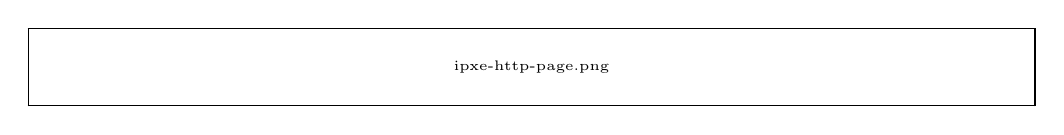
\begin{tikzpicture}
    \begin{scope}[on background layer]
      \pgftext[at=\pgfpoint{0cm}{0cm},left,base]{\pgfuseimage{httppageimg}}
    \end{scope}
  \end{tikzpicture}
  \newpage
  % arch ipxe page forcus download
  
\begin{tikzpicture}
    \fill [rounded corners=0.05mm,color=YellowOrange,nearly transparent]
      (0.3cm, 2.3cm) rectangle ++(4cm, 2.7cm); 
    \draw [rounded corners=0.05mm,color=YellowOrange]
      (0.3cm, 2.3cm) rectangle ++(4cm, 2.7cm); 
    \begin{scope}[on background layer]
      \pgftext[at=\pgfpoint{0cm}{0cm},left,base]{\pgfuseimage{httppageimg}}
    \end{scope}
  \end{tikzpicture}
  \newpage
  % arch ipxe page mark 
  \begin{tikzpicture}
    \fill [rounded corners=0.05mm,color=YellowOrange,semitransparent]
      (0.62cm, 3.2cm) rectangle ++(0.73cm, 0.2cm); 
    \draw [rounded corners=0.05mm,color=YellowOrange]
      (0.62cm, 3.2cm) rectangle ++(0.73cm, 0.2cm); 
    \begin{scope}[on background layer]
      \pgftext[at=\pgfpoint{0cm}{0cm},left,base]{\pgfuseimage{httppageimg}}
    \end{scope}
  \end{tikzpicture}

\end{document}

% vi: se ts=2 sw=2 et:
